\documentclass[10pt,a4paper]{article}

\usepackage[spanish,activeacute,es-tabla]{babel}
\usepackage[utf8]{inputenc}
\usepackage{ifthen}
\usepackage{listings}
\usepackage{dsfont}
\usepackage{subcaption}
\usepackage{amsmath}
\usepackage[strict]{changepage}
\usepackage[top=1cm,bottom=2cm,left=1cm,right=1cm]{geometry}%
\usepackage{color}%
\newcommand{\tocarEspacios}{%
	\addtolength{\leftskip}{3em}%
	\setlength{\parindent}{0em}%
}

% Especificacion de procs

\newcommand{\In}{\textsf{in }}
\newcommand{\Out}{\textsf{out }}
\newcommand{\Inout}{\textsf{inout }}

\newcommand{\encabezadoDeProc}[4]{%
	% Ponemos la palabrita problema en tt
	%  \noindent%
	{\normalfont\bfseries\ttfamily proc}%
	% Ponemos el nombre del problema
	\ %
	{\normalfont\ttfamily #2}%
	\
	% Ponemos los parametros
	(#3)%
	\ifthenelse{\equal{#4}{}}{}{%
		% Por ultimo, va el tipo del resultado
		\ : #4}
}

\newenvironment{proc}[4][res]{%
	
	% El parametro 1 (opcional) es el nombre del resultado
	% El parametro 2 es el nombre del problema
	% El parametro 3 son los parametros
	% El parametro 4 es el tipo del resultado
	% Preambulo del ambiente problema
	% Tenemos que definir los comandos requiere, asegura, modifica y aux
	\newcommand{\requiere}[2][]{%
		{\normalfont\bfseries\ttfamily requiere}%
		\ifthenelse{\equal{##1}{}}{}{\ {\normalfont\ttfamily ##1} :}\ %
		\{\ensuremath{##2}\}%
		{\normalfont\bfseries\,\par}%
	}
	\newcommand{\asegura}[2][]{%
		{\normalfont\bfseries\ttfamily asegura}%
		\ifthenelse{\equal{##1}{}}{}{\ {\normalfont\ttfamily ##1} :}\
		\{\ensuremath{##2}\}%
		{\normalfont\bfseries\,\par}%
	}
	\renewcommand{\aux}[4]{%
		{\normalfont\bfseries\ttfamily aux\ }%
		{\normalfont\ttfamily ##1}%
		\ifthenelse{\equal{##2}{}}{}{\ (##2)}\ : ##3\, = \ensuremath{##4}%
		{\normalfont\bfseries\,;\par}%
	}
	\renewcommand{\pred}[3]{%
		{\normalfont\bfseries\ttfamily pred }%
		{\normalfont\ttfamily ##1}%
		\ifthenelse{\equal{##2}{}}{}{\ (##2) }%
		\{%
		\begin{adjustwidth}{+5em}{}
			\ensuremath{##3}
		\end{adjustwidth}
		\}%
		{\normalfont\bfseries\,\par}%
	}
	
	\newcommand{\res}{#1}
	\vspace{1ex}
	\noindent
	\encabezadoDeProc{#1}{#2}{#3}{#4}
	% Abrimos la llave
	\par%
	\tocarEspacios
}
{
	% Cerramos la llave
	\vspace{1ex}
}

\newcommand{\aux}[4]{%
	{\normalfont\bfseries\ttfamily\noindent aux\ }%
	{\normalfont\ttfamily #1}%
	\ifthenelse{\equal{#2}{}}{}{\ (#2)}\ : #3\, = \ensuremath{#4}%
	{\normalfont\bfseries\,;\par}%
}

\newcommand{\pred}[3]{%
	{\normalfont\bfseries\ttfamily\noindent pred }%
	{\normalfont\ttfamily #1}%
	\ifthenelse{\equal{#2}{}}{}{\ (#2) }%
	\{%
	\begin{adjustwidth}{+2em}{}
		\ensuremath{#3}
	\end{adjustwidth}
	\}%
	{\normalfont\bfseries\,\par}%
}

% Tipos

\newcommand{\nat}{\ensuremath{\mathds{N}}}
\newcommand{\ent}{\ensuremath{\mathds{Z}}}
\newcommand{\float}{\ensuremath{\mathds{R}}}
\newcommand{\bool}{\ensuremath{\mathsf{Bool}}}
\newcommand{\cha}{\ensuremath{\mathsf{Char}}}
\newcommand{\str}{\ensuremath{\mathsf{String}}}

% Logica

\newcommand{\True}{\ensuremath{\mathrm{true}}}
\newcommand{\False}{\ensuremath{\mathrm{false}}}
\newcommand{\Then}{\ensuremath{\rightarrow}}
\newcommand{\Iff}{\ensuremath{\leftrightarrow}}
\newcommand{\implica}{\ensuremath{\longrightarrow}}
\newcommand{\IfThenElse}[3]{\ensuremath{\mathsf{if}\ #1\ \mathsf{then}\ #2\ \mathsf{else}\ #3\ \mathsf{fi}}}
\newcommand{\yLuego}{\land _L}
\newcommand{\oLuego}{\lor _L}
\newcommand{\implicaLuego}{\implica _L}

\newcommand{\cuantificador}[5]{%
	\ensuremath{(#2 #3: #4)\ (%
		\ifthenelse{\equal{#1}{unalinea}}{
			#5
		}{
			$ % exiting math mode
			\begin{adjustwidth}{+2em}{}
				$#5$%
			\end{adjustwidth}%
			$ % entering math mode
		}
		)}
}

\newcommand{\existe}[4][]{%
	\cuantificador{#1}{\exists}{#2}{#3}{#4}
}
\newcommand{\paraTodo}[4][]{%
	\cuantificador{#1}{\forall}{#2}{#3}{#4}
}

%listas

\newcommand{\TLista}[1]{\ensuremath{seq \langle #1\rangle}}
\newcommand{\lvacia}{\ensuremath{[\ ]}}
\newcommand{\lv}{\ensuremath{[\ ]}}
\newcommand{\longitud}[1]{\ensuremath{|#1|}}
\newcommand{\cons}[1]{\ensuremath{\mathsf{addFirst}}(#1)}
\newcommand{\indice}[1]{\ensuremath{\mathsf{indice}}(#1)}
\newcommand{\conc}[1]{\ensuremath{\mathsf{concat}}(#1)}
\newcommand{\cab}[1]{\ensuremath{\mathsf{head}}(#1)}
\newcommand{\cola}[1]{\ensuremath{\mathsf{tail}}(#1)}
\newcommand{\sub}[1]{\ensuremath{\mathsf{subseq}}(#1)}
\newcommand{\en}[1]{\ensuremath{\mathsf{en}}(#1)}
\newcommand{\cuenta}[2]{\mathsf{cuenta}\ensuremath{(#1, #2)}}
\newcommand{\suma}[1]{\mathsf{suma}(#1)}
\newcommand{\twodots}{\ensuremath{\mathrm{..}}}
\newcommand{\masmas}{\ensuremath{++}}
\newcommand{\matriz}[1]{\TLista{\TLista{#1}}}
\newcommand{\seqchar}{\TLista{\cha}}

\renewcommand{\lstlistingname}{Código}
\lstset{% general command to set parameter(s)
	language=Java,
	morekeywords={endif, endwhile, skip},
	basewidth={0.47em,0.40em},
	columns=fixed, fontadjust, resetmargins, xrightmargin=5pt, xleftmargin=15pt,
	flexiblecolumns=false, tabsize=4, breaklines, breakatwhitespace=false, extendedchars=true,
	numbers=left, numberstyle=\tiny, stepnumber=1, numbersep=9pt,
	frame=l, framesep=3pt,
	captionpos=b,
}

\usepackage{caratula} % Version modificada para usar las macros de algo1 de ~> https://github.com/bcardiff/dc-tex


\titulo{Trabajo Práctico 2}
\subtitulo{Clasificación y Selección de Modelos}

\fecha{\today}

\materia{Laboratorio de Datos}
\grupo{Grupo 100}

\integrante{Apellido, Nombre1}{001/01}{email1@dominio.com}
\integrante{Martinelli, Lorenzo}{364/23}{martinelli.lorenzo12@gmail.com}
\integrante{Padilla, Ramiro}{1636/21}{ramiromdq123@gmail.com}
% Pongan cuantos integrantes quieran

% Declaramos donde van a estar las figuras
% No es obligatorio, pero suele ser comodo
\graphicspath{{../static/}}

\begin{document}

\maketitle

\section{Introducción}  \vspace{0.1cm}

\subsection{Fuente de datos} \vspace{0.1cm}

A lo largo de este proyecto, trabajaremos con un conjunto de datos de imágenes denominado Sign
Language MNIST, el cual se encuentra en formato csv, donde cada imagen del set de datos representa una letra en lenguaje de
señas americano. El link al dataset es el siguiente https://www.kaggle.com/datasets/datamunge/sign-language-mnist.

\subsection{Análisis exploratorio de datos}  \vspace{0.1cm}

Antes de ponernos a trabajar con los datos, necesitamos saber mas acerca de ellos. Sabemos que, cada fila del dataset representa una imagen de 28x28 pixeles en escala de grises que corresponde a una letra en lenguaje de señas, miremos a continuación un pequeño fragmento del mismo.

 \vspace{0.1cm}

\begin{figure}[h]
  \centering
  \includegraphics[width=1.0\textwidth]{Imagenes/atributos\_relevantes.png}
  \caption{Primeras nueve imagenes del dataset}
  \label{fig:Tabla 1}
\end{figure}

 \vspace{0.1cm}

A partir del gráfico anterior, podemos inferir que no todos los pixeles son realmente relevante para diferenciar imágenes entre si. Por ejemplo, podemos ver
que aquellos pixeles correspondientes al fondo no aportan información alguna. ¿Cuántos pixeles necesitaremos realmente para diferenciar las imágenes? \vspace{0.05cm}

Por otro lado, viendo por ejemplo, que las letras C y D aparecen más de una vez, también surge la pregunta. ¿Están balanceadas las distintas clases que identifican a las letras? En el gráfico a continuación, podremos notar que tenemos un dataset con una excelente distribución de clases. ¿Por qué me interesa
tener una cantidad pareja de cada muestra? Esto, adquiere relevancia puesto que al entrenar nuestros modelos en un futuro, no queremos tener sesgos.
\vspace{0.05cm}
  
Obs: Las letras J y Z no poseen ningún ejemplar puesto que requieren de movimiento para su seña.

\vspace{0.1cm}

\begin{figure}[h]
  \centering
  \includegraphics[width=0.8\textwidth]{Imagenes/distribucion.png}
  \caption{Cantidad de muestras de cada letra}
  \label{fig:Tabla 1}
\end{figure}

\newpage

Otra pregunta que naturalmente surge al explorar el dataser es que tan distintas son las letras entre sí, y si las diferentes muestras respecto a una misma letras
presentan diferencias notorias o no. Para eso, comparemos por ejemplo, las letras E, L Y M.

\begin{figure}[ht!]
	\begin{subfigure}{0.5\textwidth}
		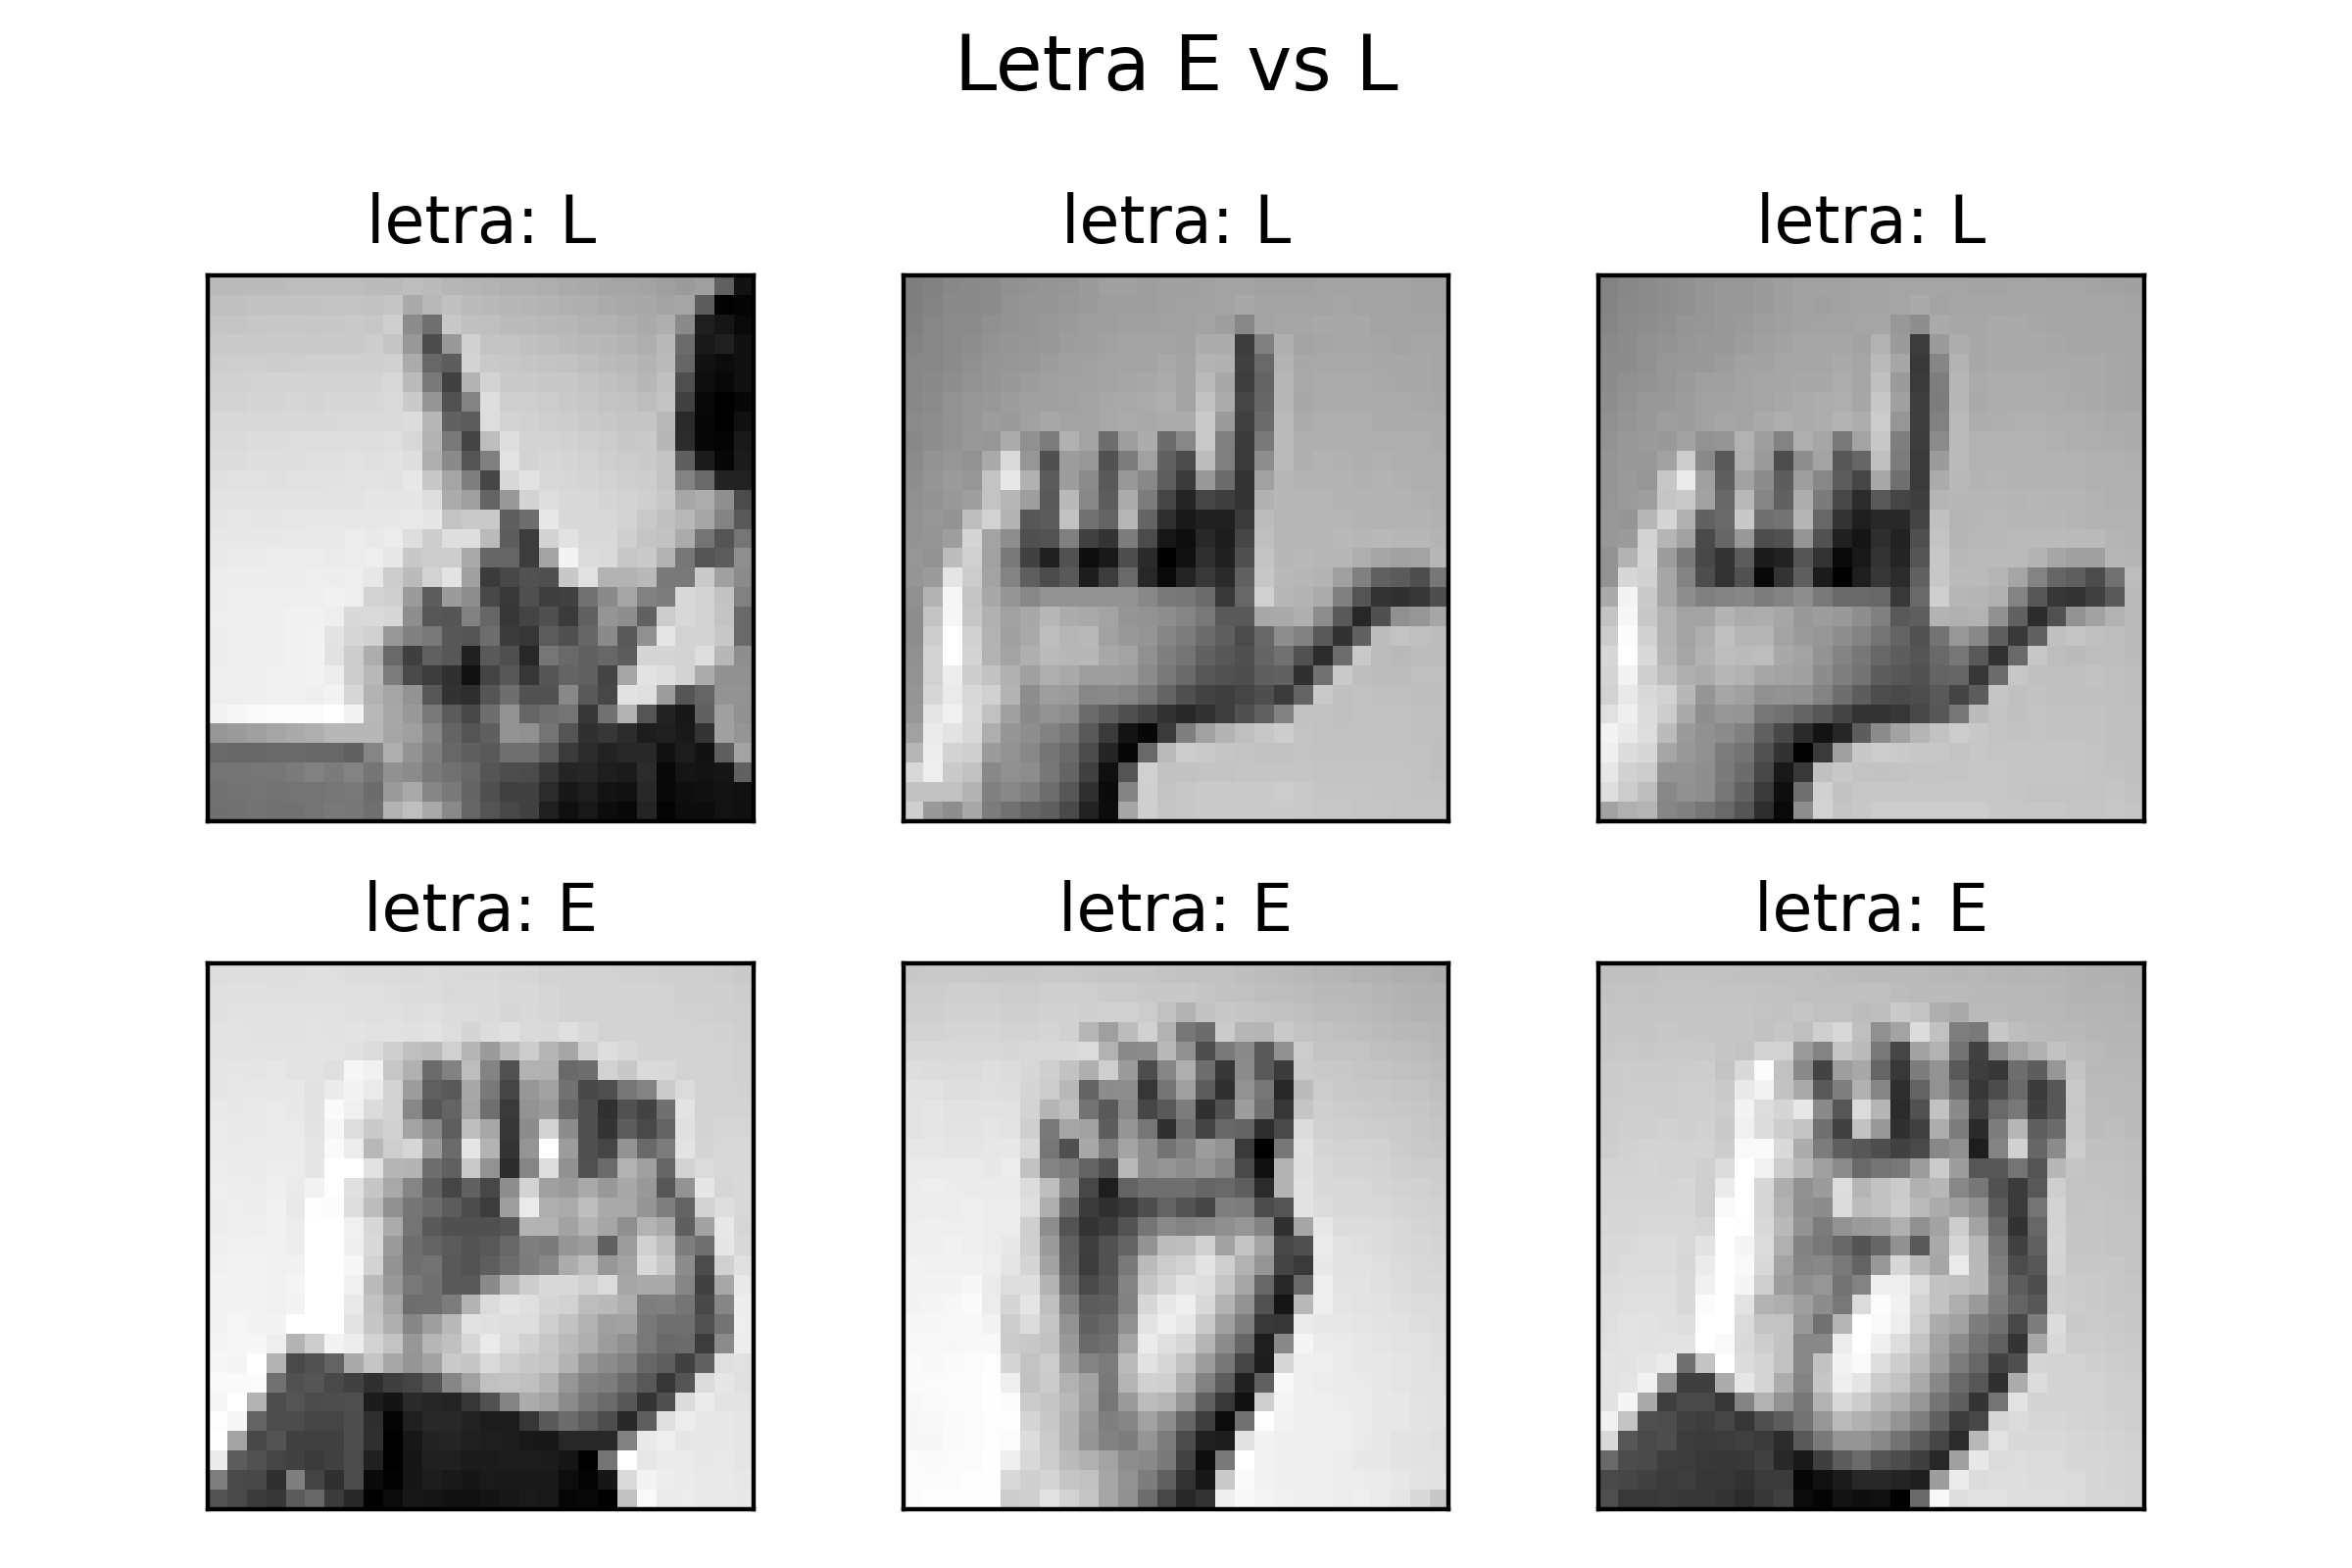
\includegraphics[width=0.9\linewidth]{Imagenes/letra_E_vs_L.png} 
		\caption{Los 3 pixeles con mayor varianza}
		\label{fig:subfig1}
	\end{subfigure}
	\begin{subfigure}{0.5\textwidth}
		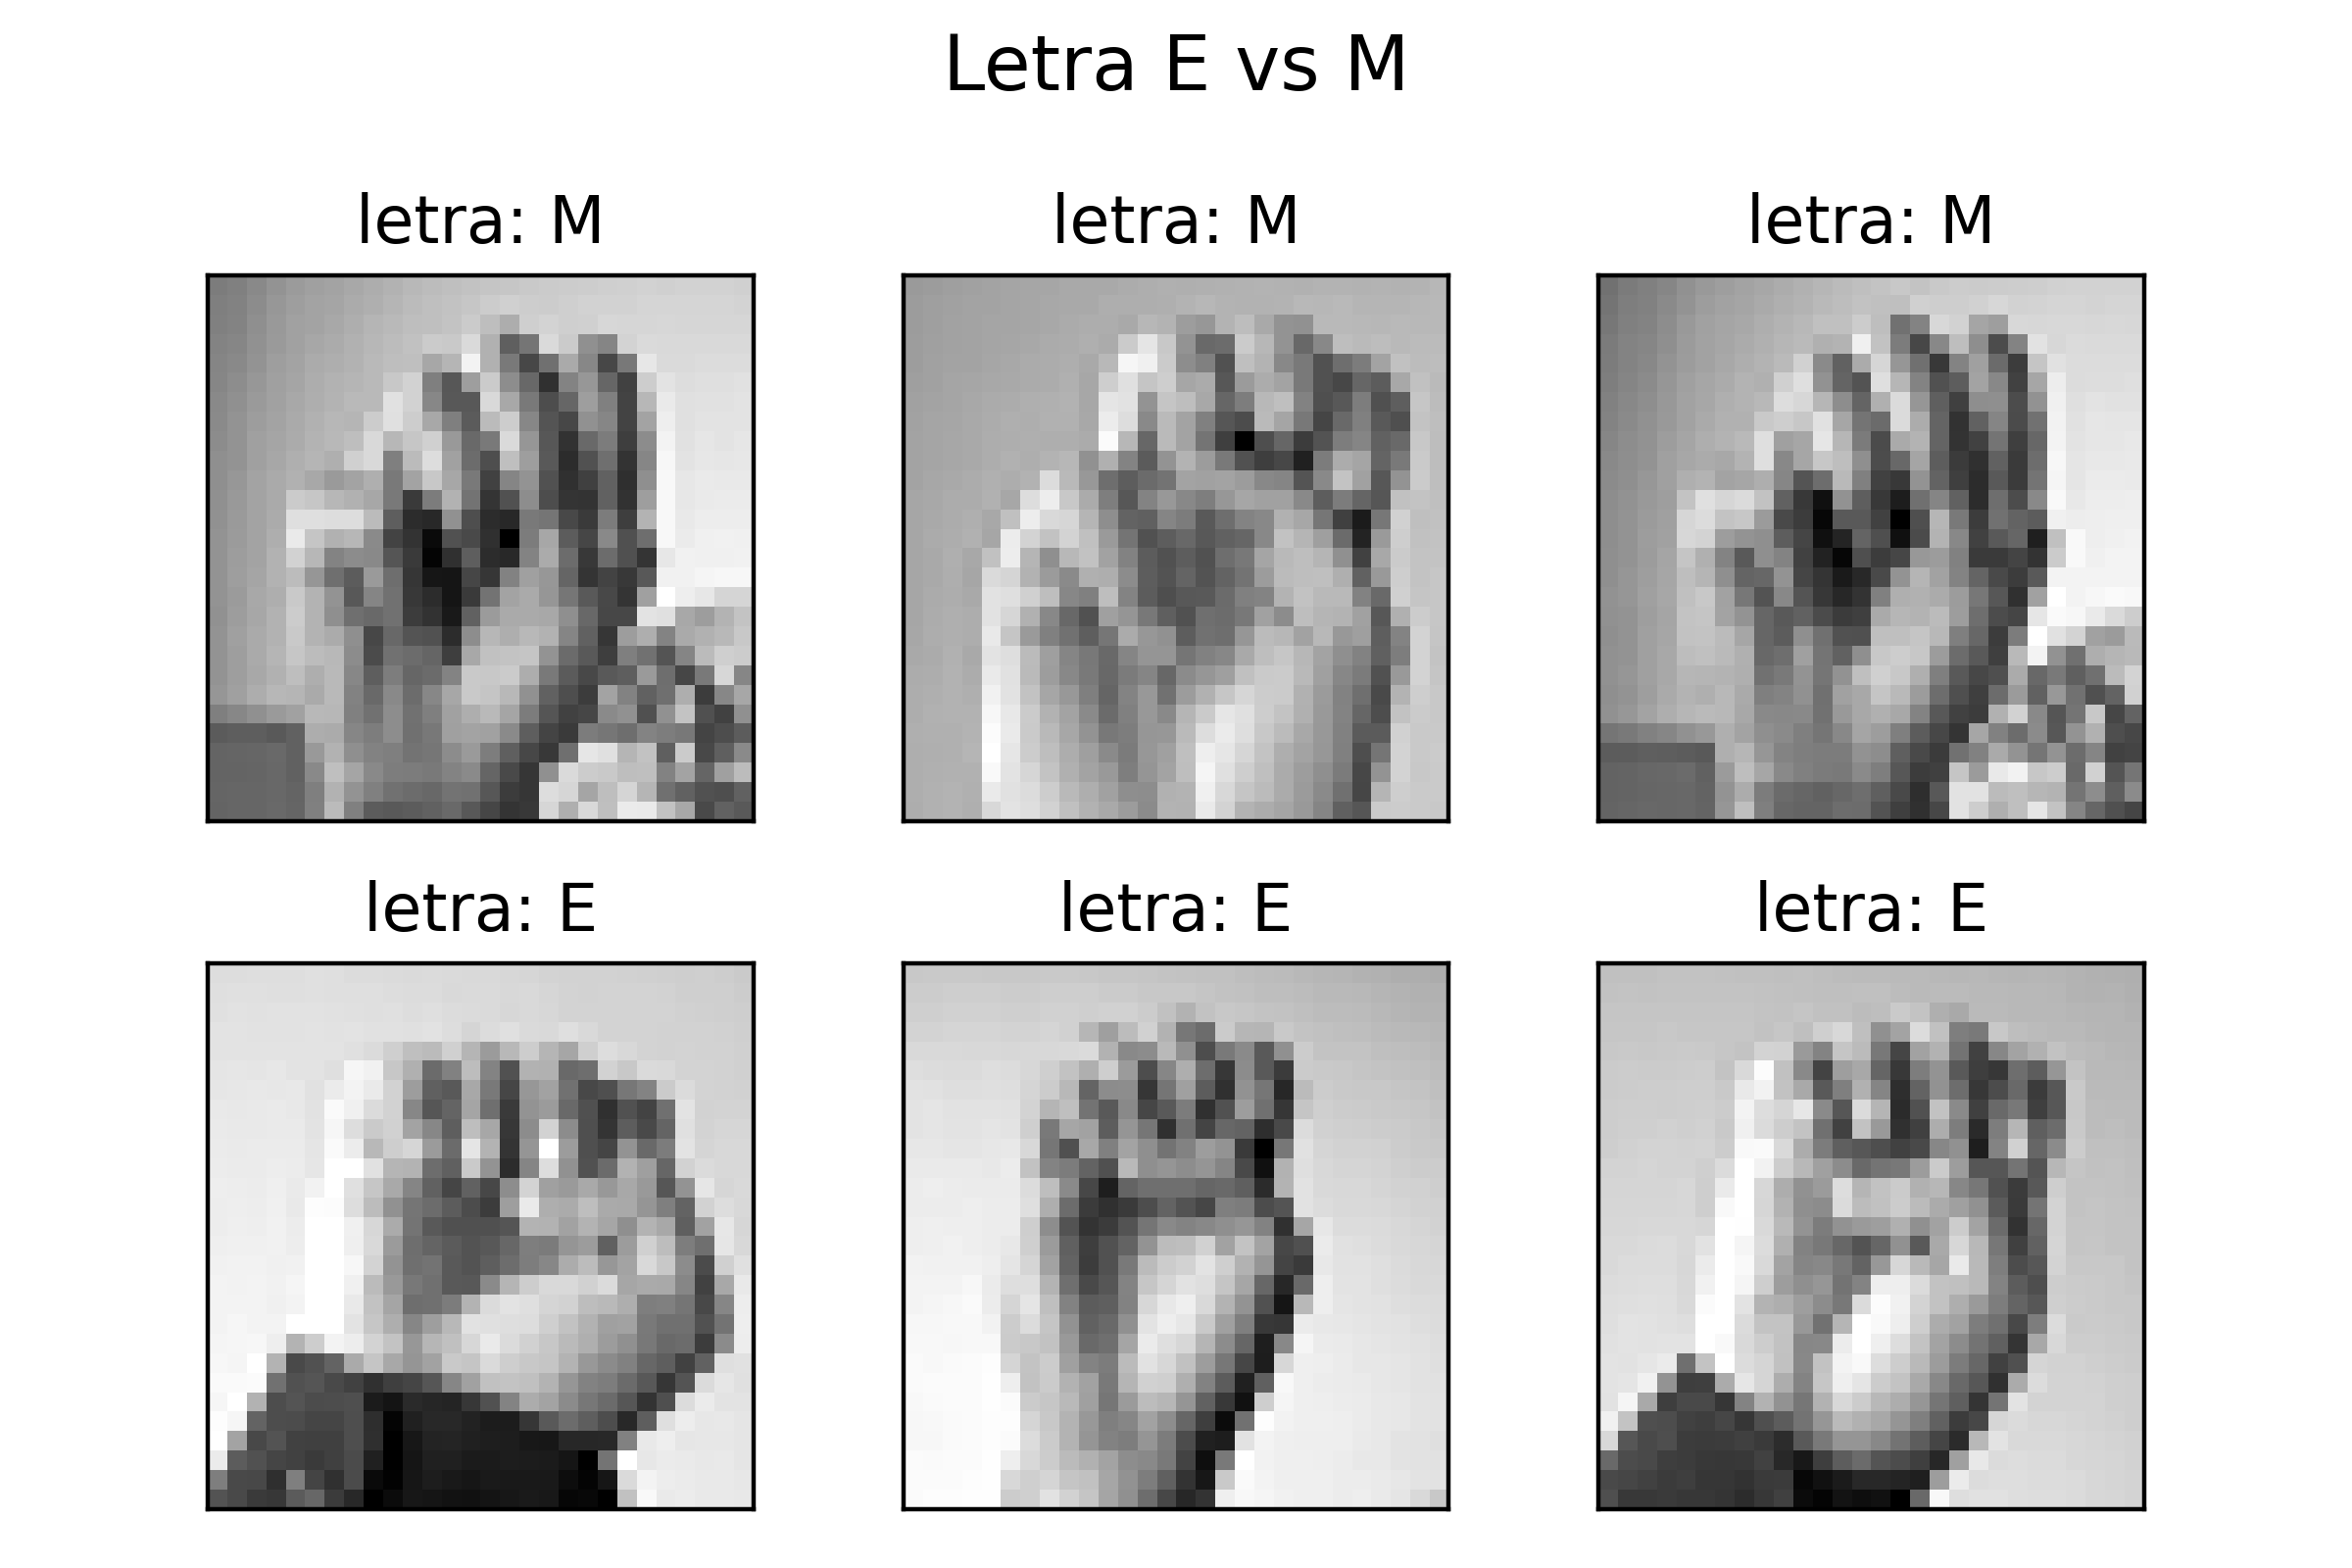
\includegraphics[width=0.9\linewidth]{Imagenes/letra_E_vs_M.png}
		\caption{50 pixeles en una zona de varianza media}
		\label{fig:subfig2}
	\end{subfigure}
	% OJO: el caption siempre va antes del label
	\label{fig:subfigs}
\end{figure}

\section{Modelo}
Realizando distintas pruebas, notamos que utilizando distintas cantidades de pixeles, a medida que el numero de vecinos incrementa
la performance decae, siendo el número ideal de vecinos exactamente 1.

\begin{figure}[ht!]
	\begin{subfigure}{0.5\textwidth}
		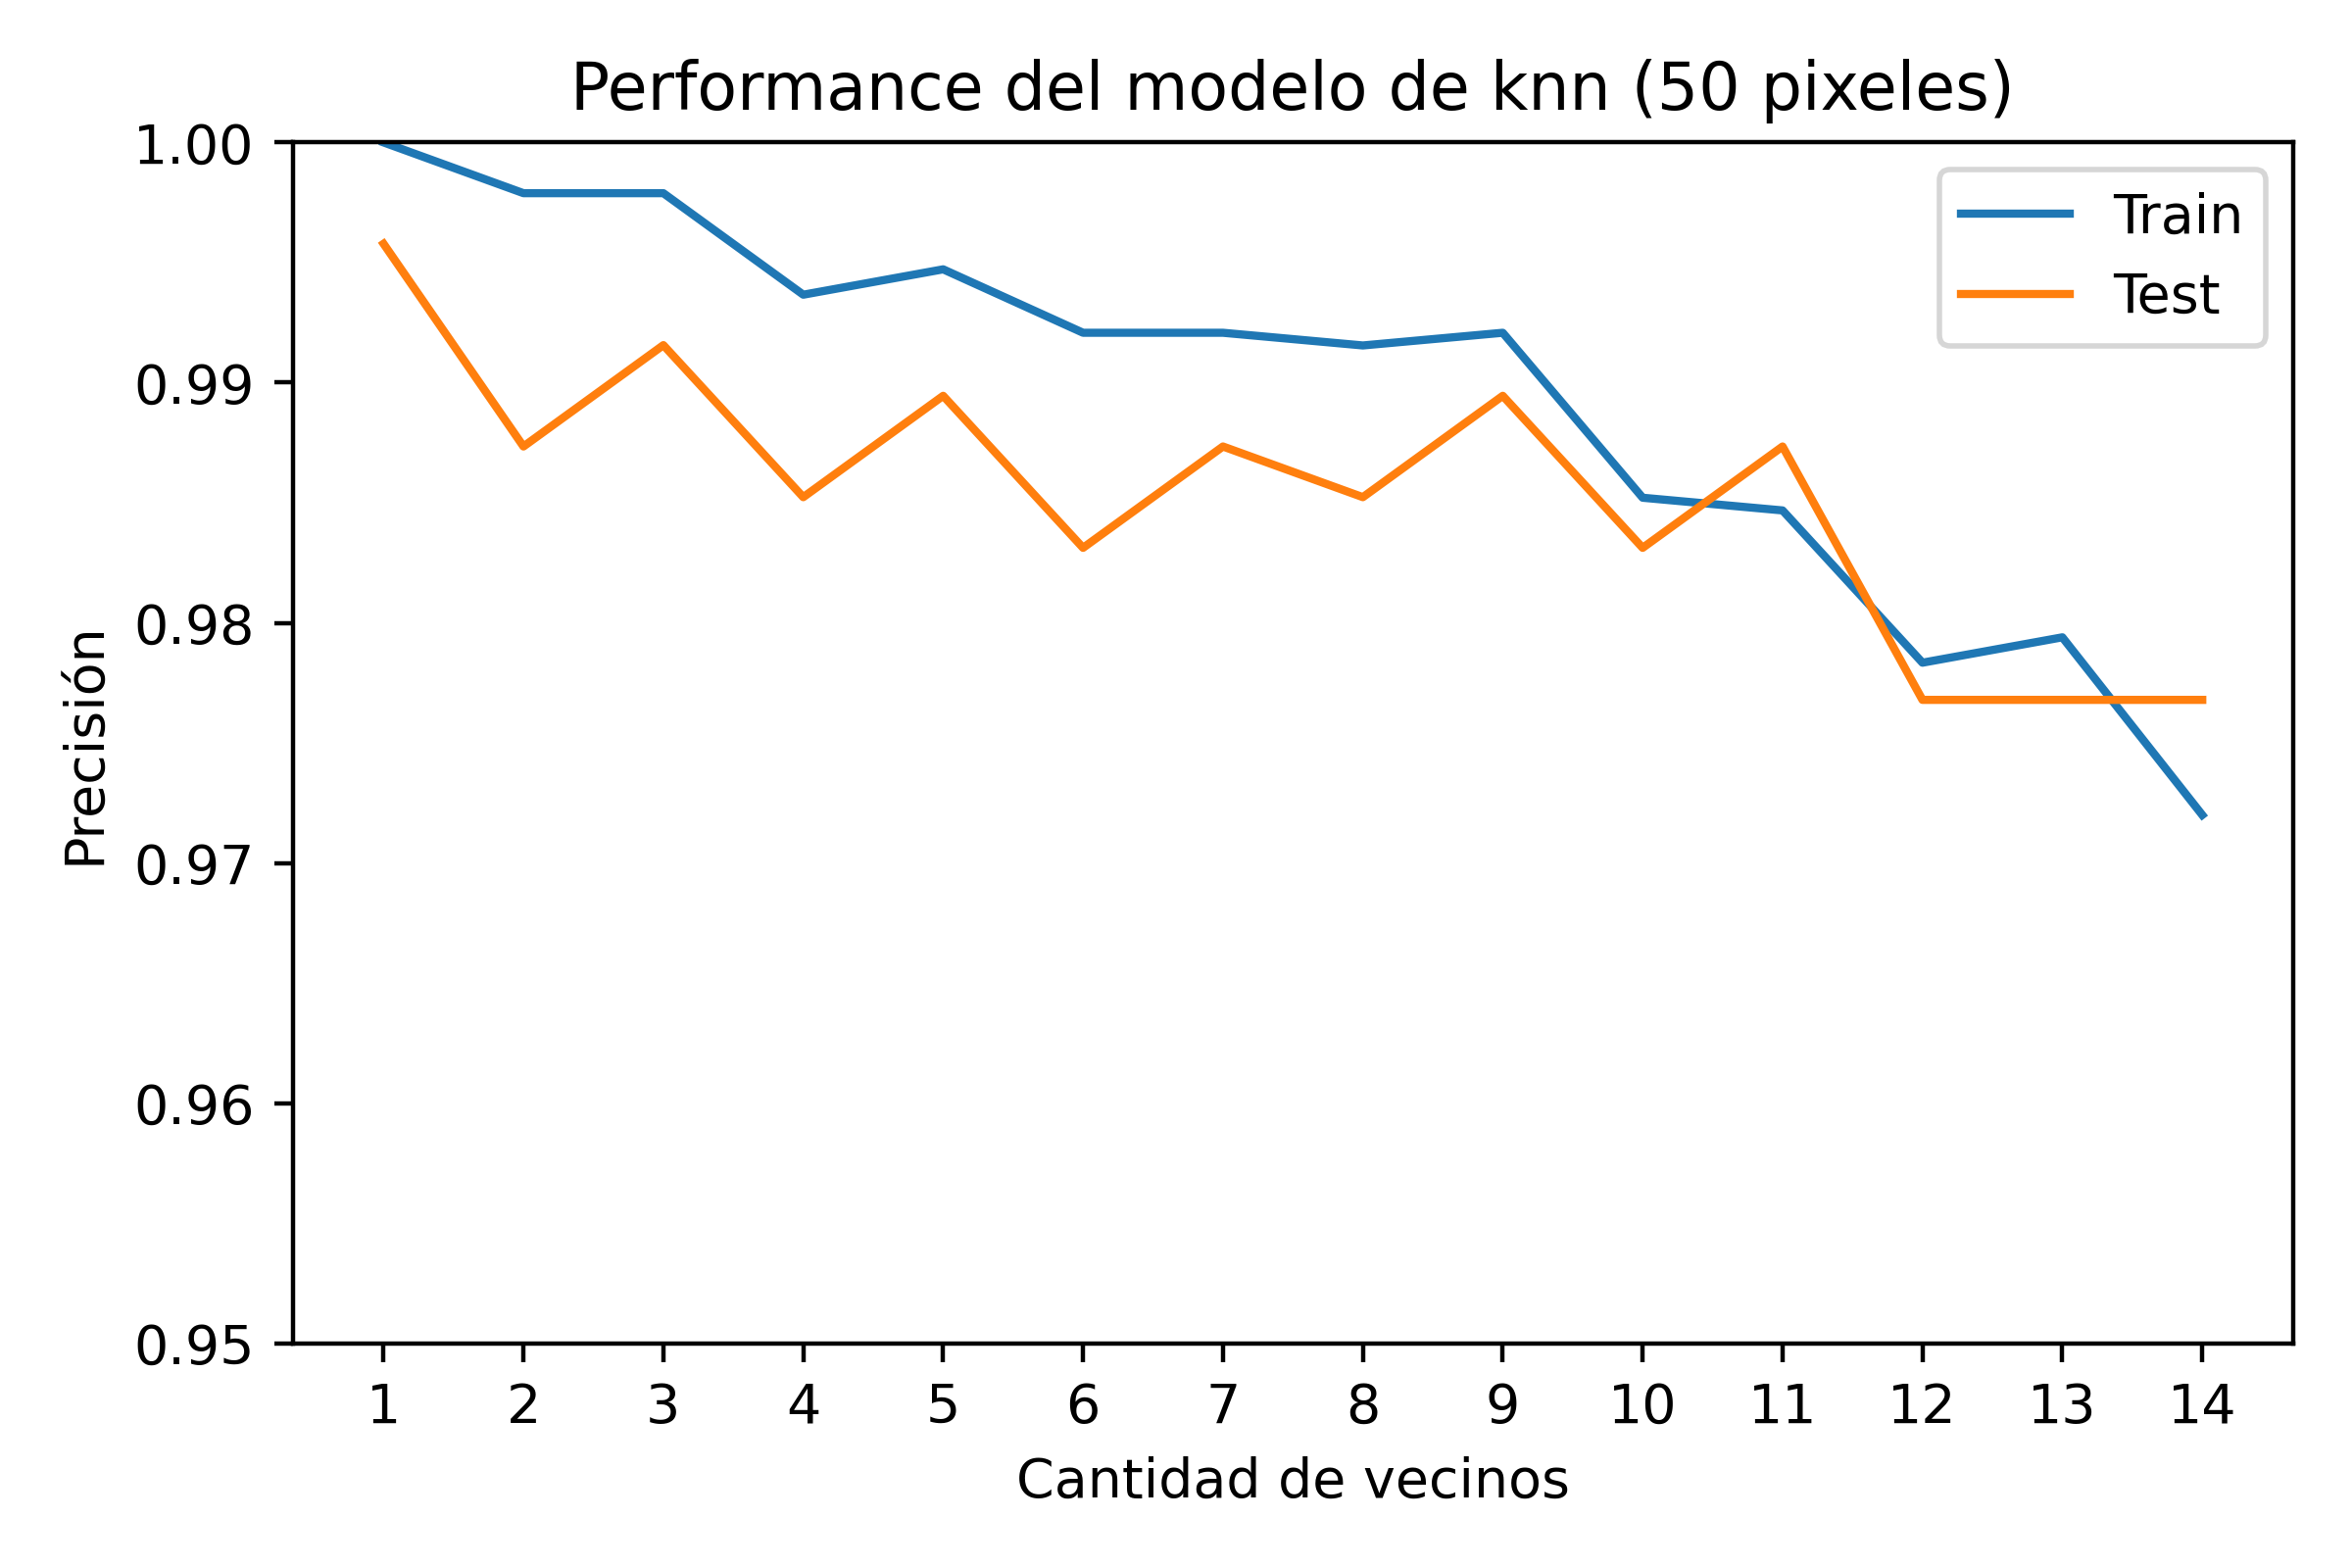
\includegraphics[width=0.9\linewidth]{Imagenes/50pixeles.png} 
		\caption{Los 3 pixeles con mayor varianza}
		\label{fig:subfig1}
	\end{subfigure}
	\begin{subfigure}{0.5\textwidth}
		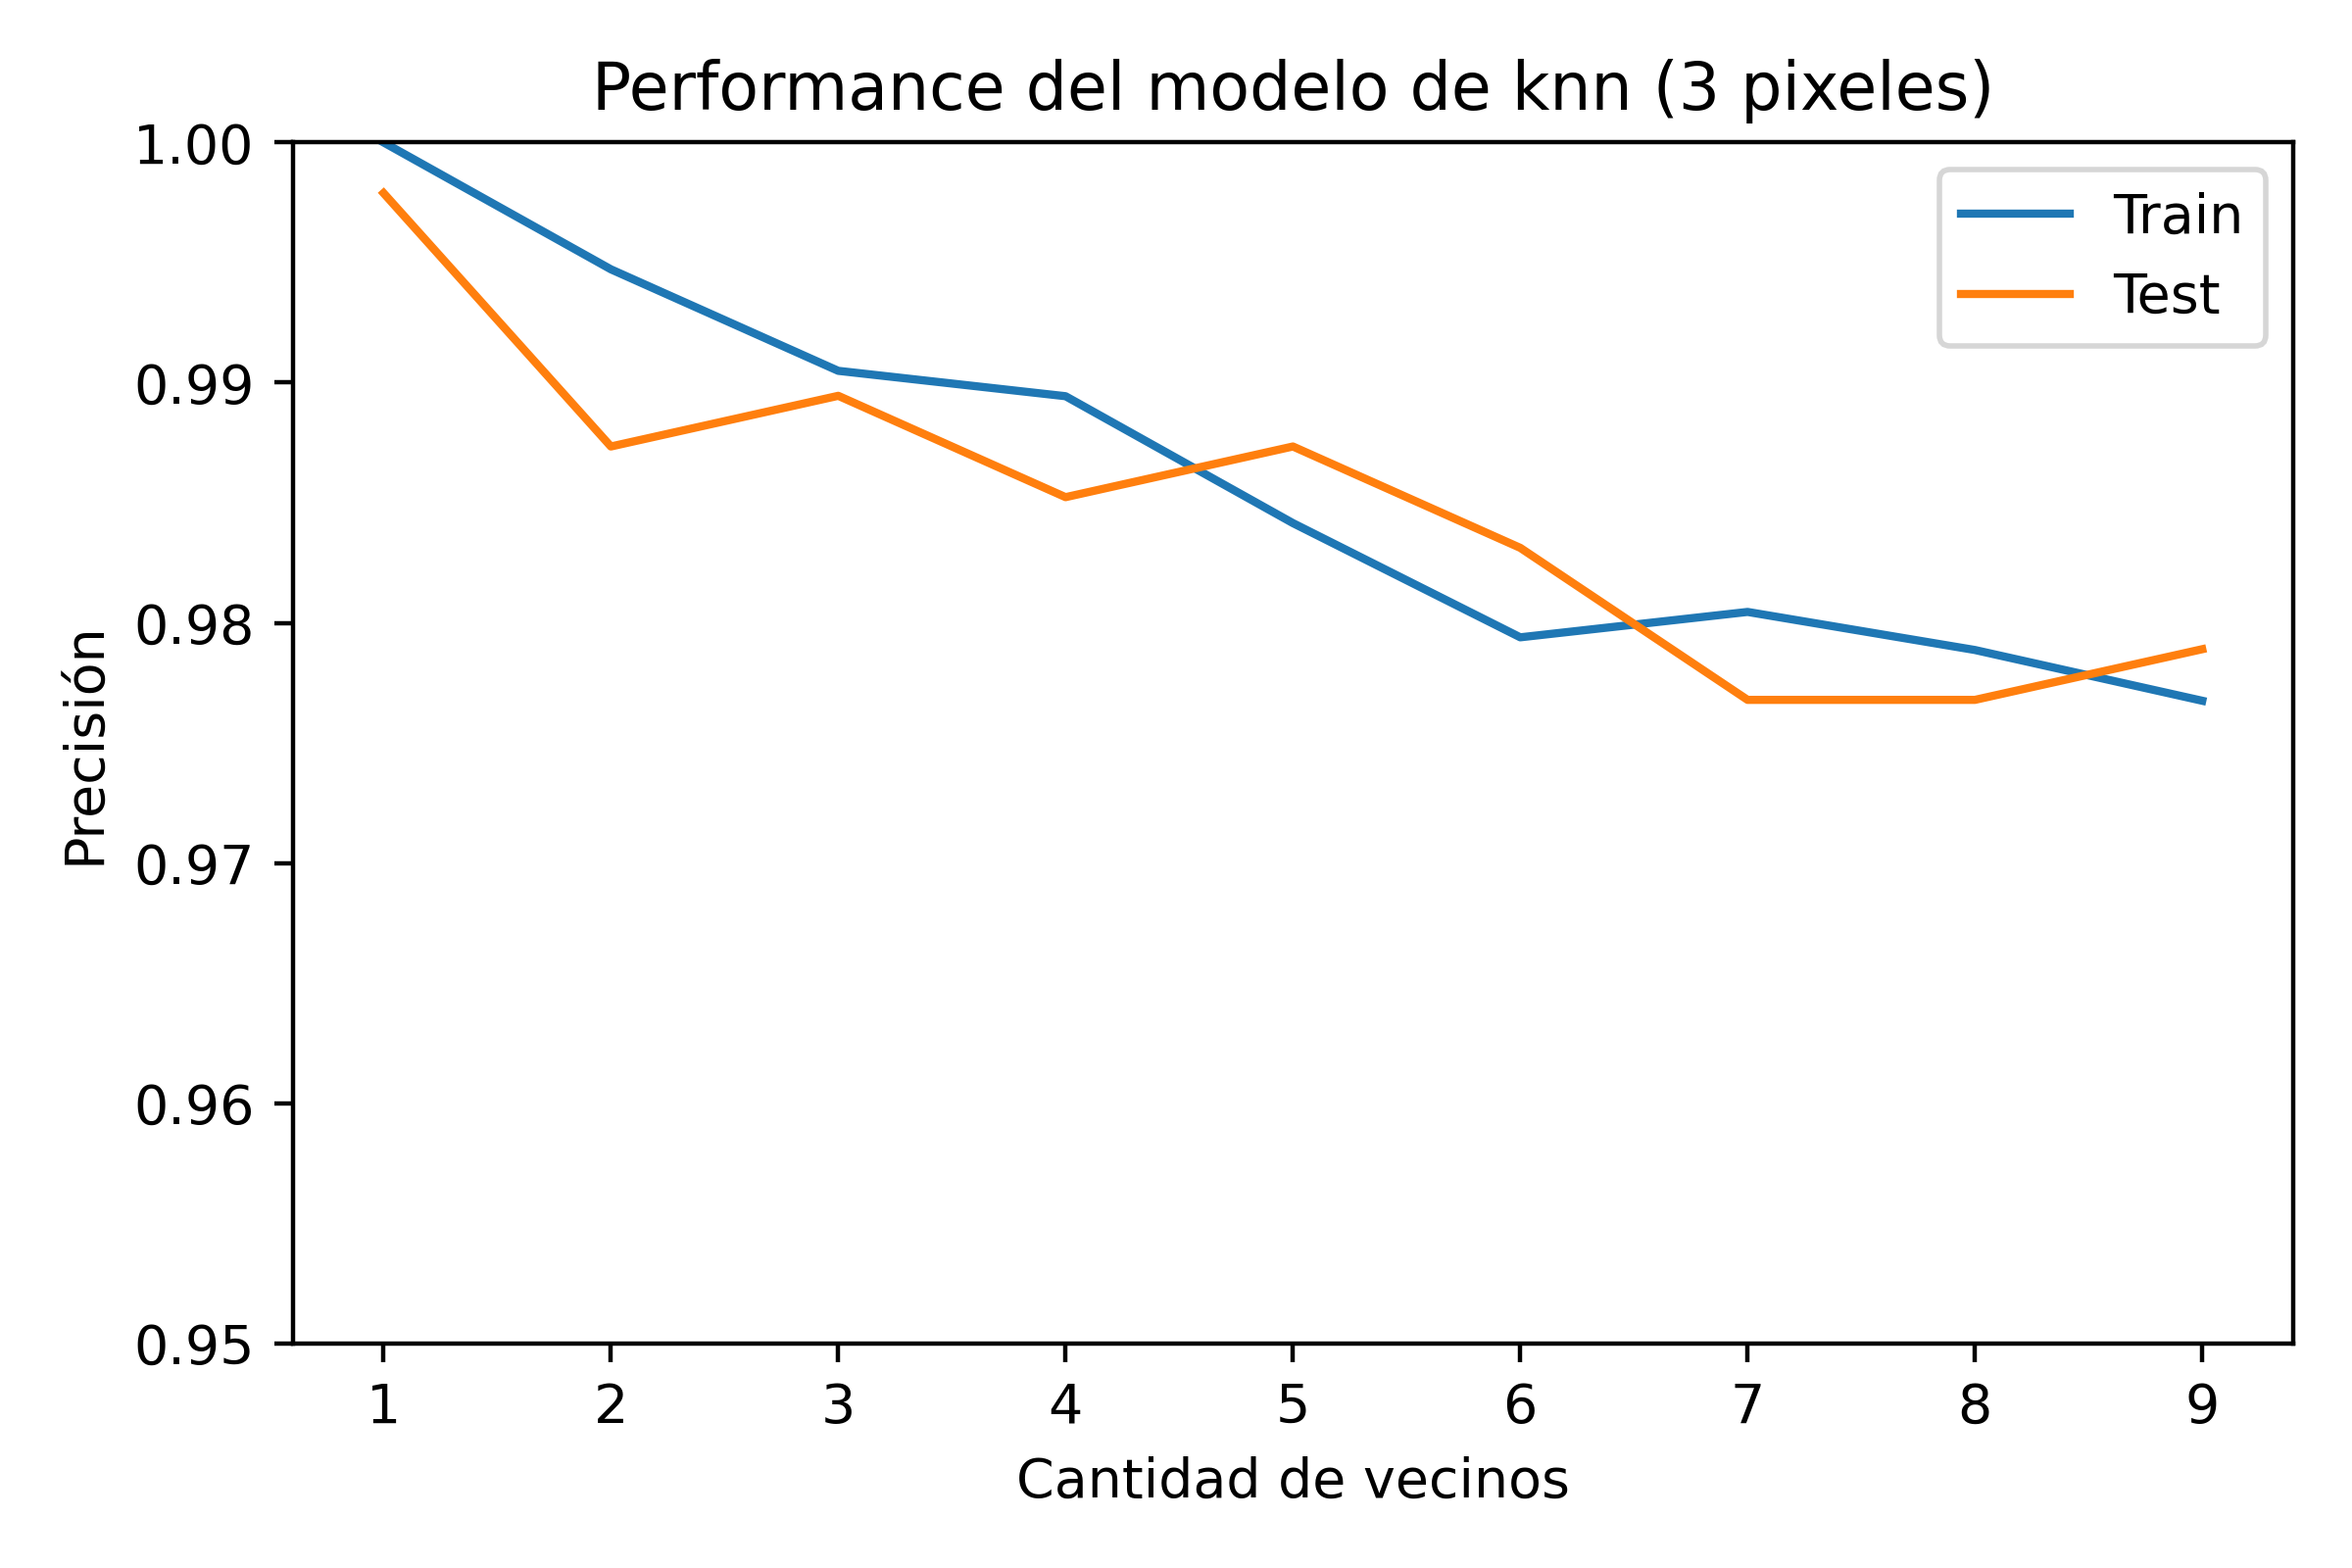
\includegraphics[width=0.9\linewidth]{Imagenes/3pixeles.png}
		\caption{50 pixeles en una zona de varianza media}
		\label{fig:subfig2}
	\end{subfigure}
	% OJO: el caption siempre va antes del label
	\label{fig:subfigs}
\end{figure}

Sin embargo, encontramos que cuando tenemos solo un pixel. Sin importar si este es significativo o no, la performance del modelo tiende a aumentar a medida
que el numero de vecinos es mayor. En este caso, a partir de los gráficos, pareciera ser que k = 9 sería un buen número.

\begin{figure}[ht!]
	\begin{subfigure}{0.5\textwidth}
		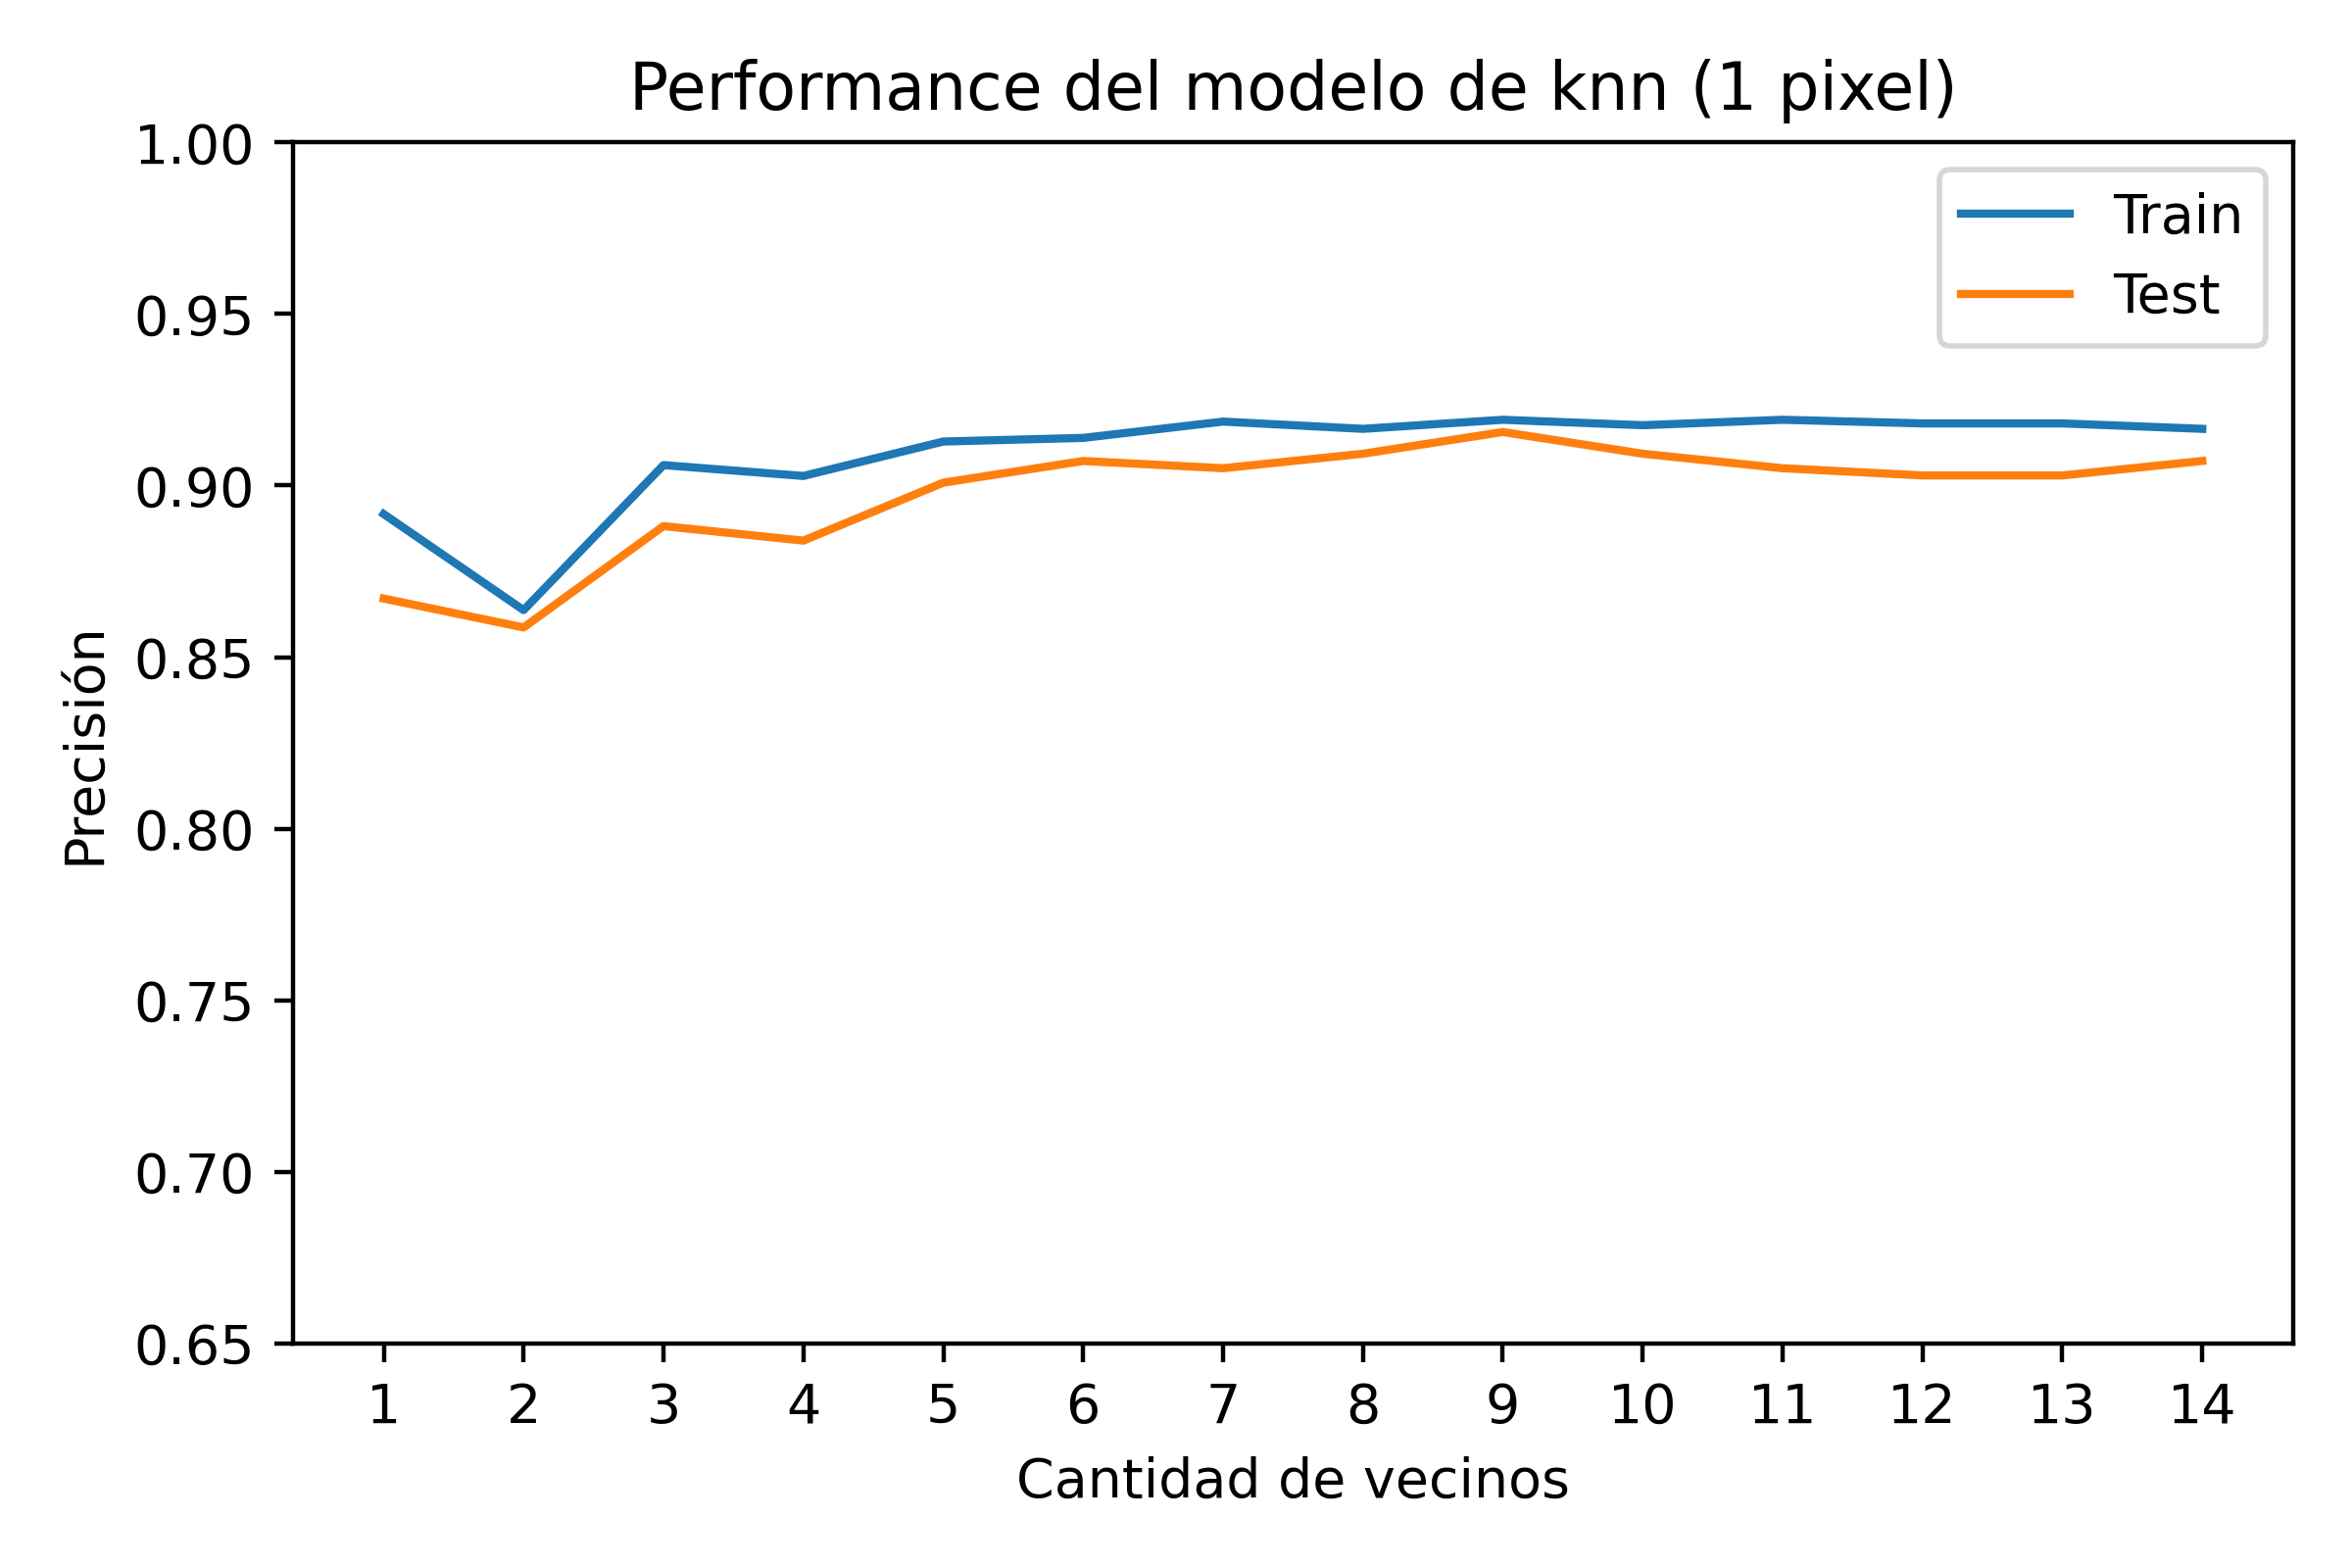
\includegraphics[width=0.9\linewidth]{imagenes/1pixelalto.png} 
		\caption{Pixeles de alta varianza}
		\label{fig:subfig1}
	\end{subfigure}
	\begin{subfigure}{0.5\textwidth}
		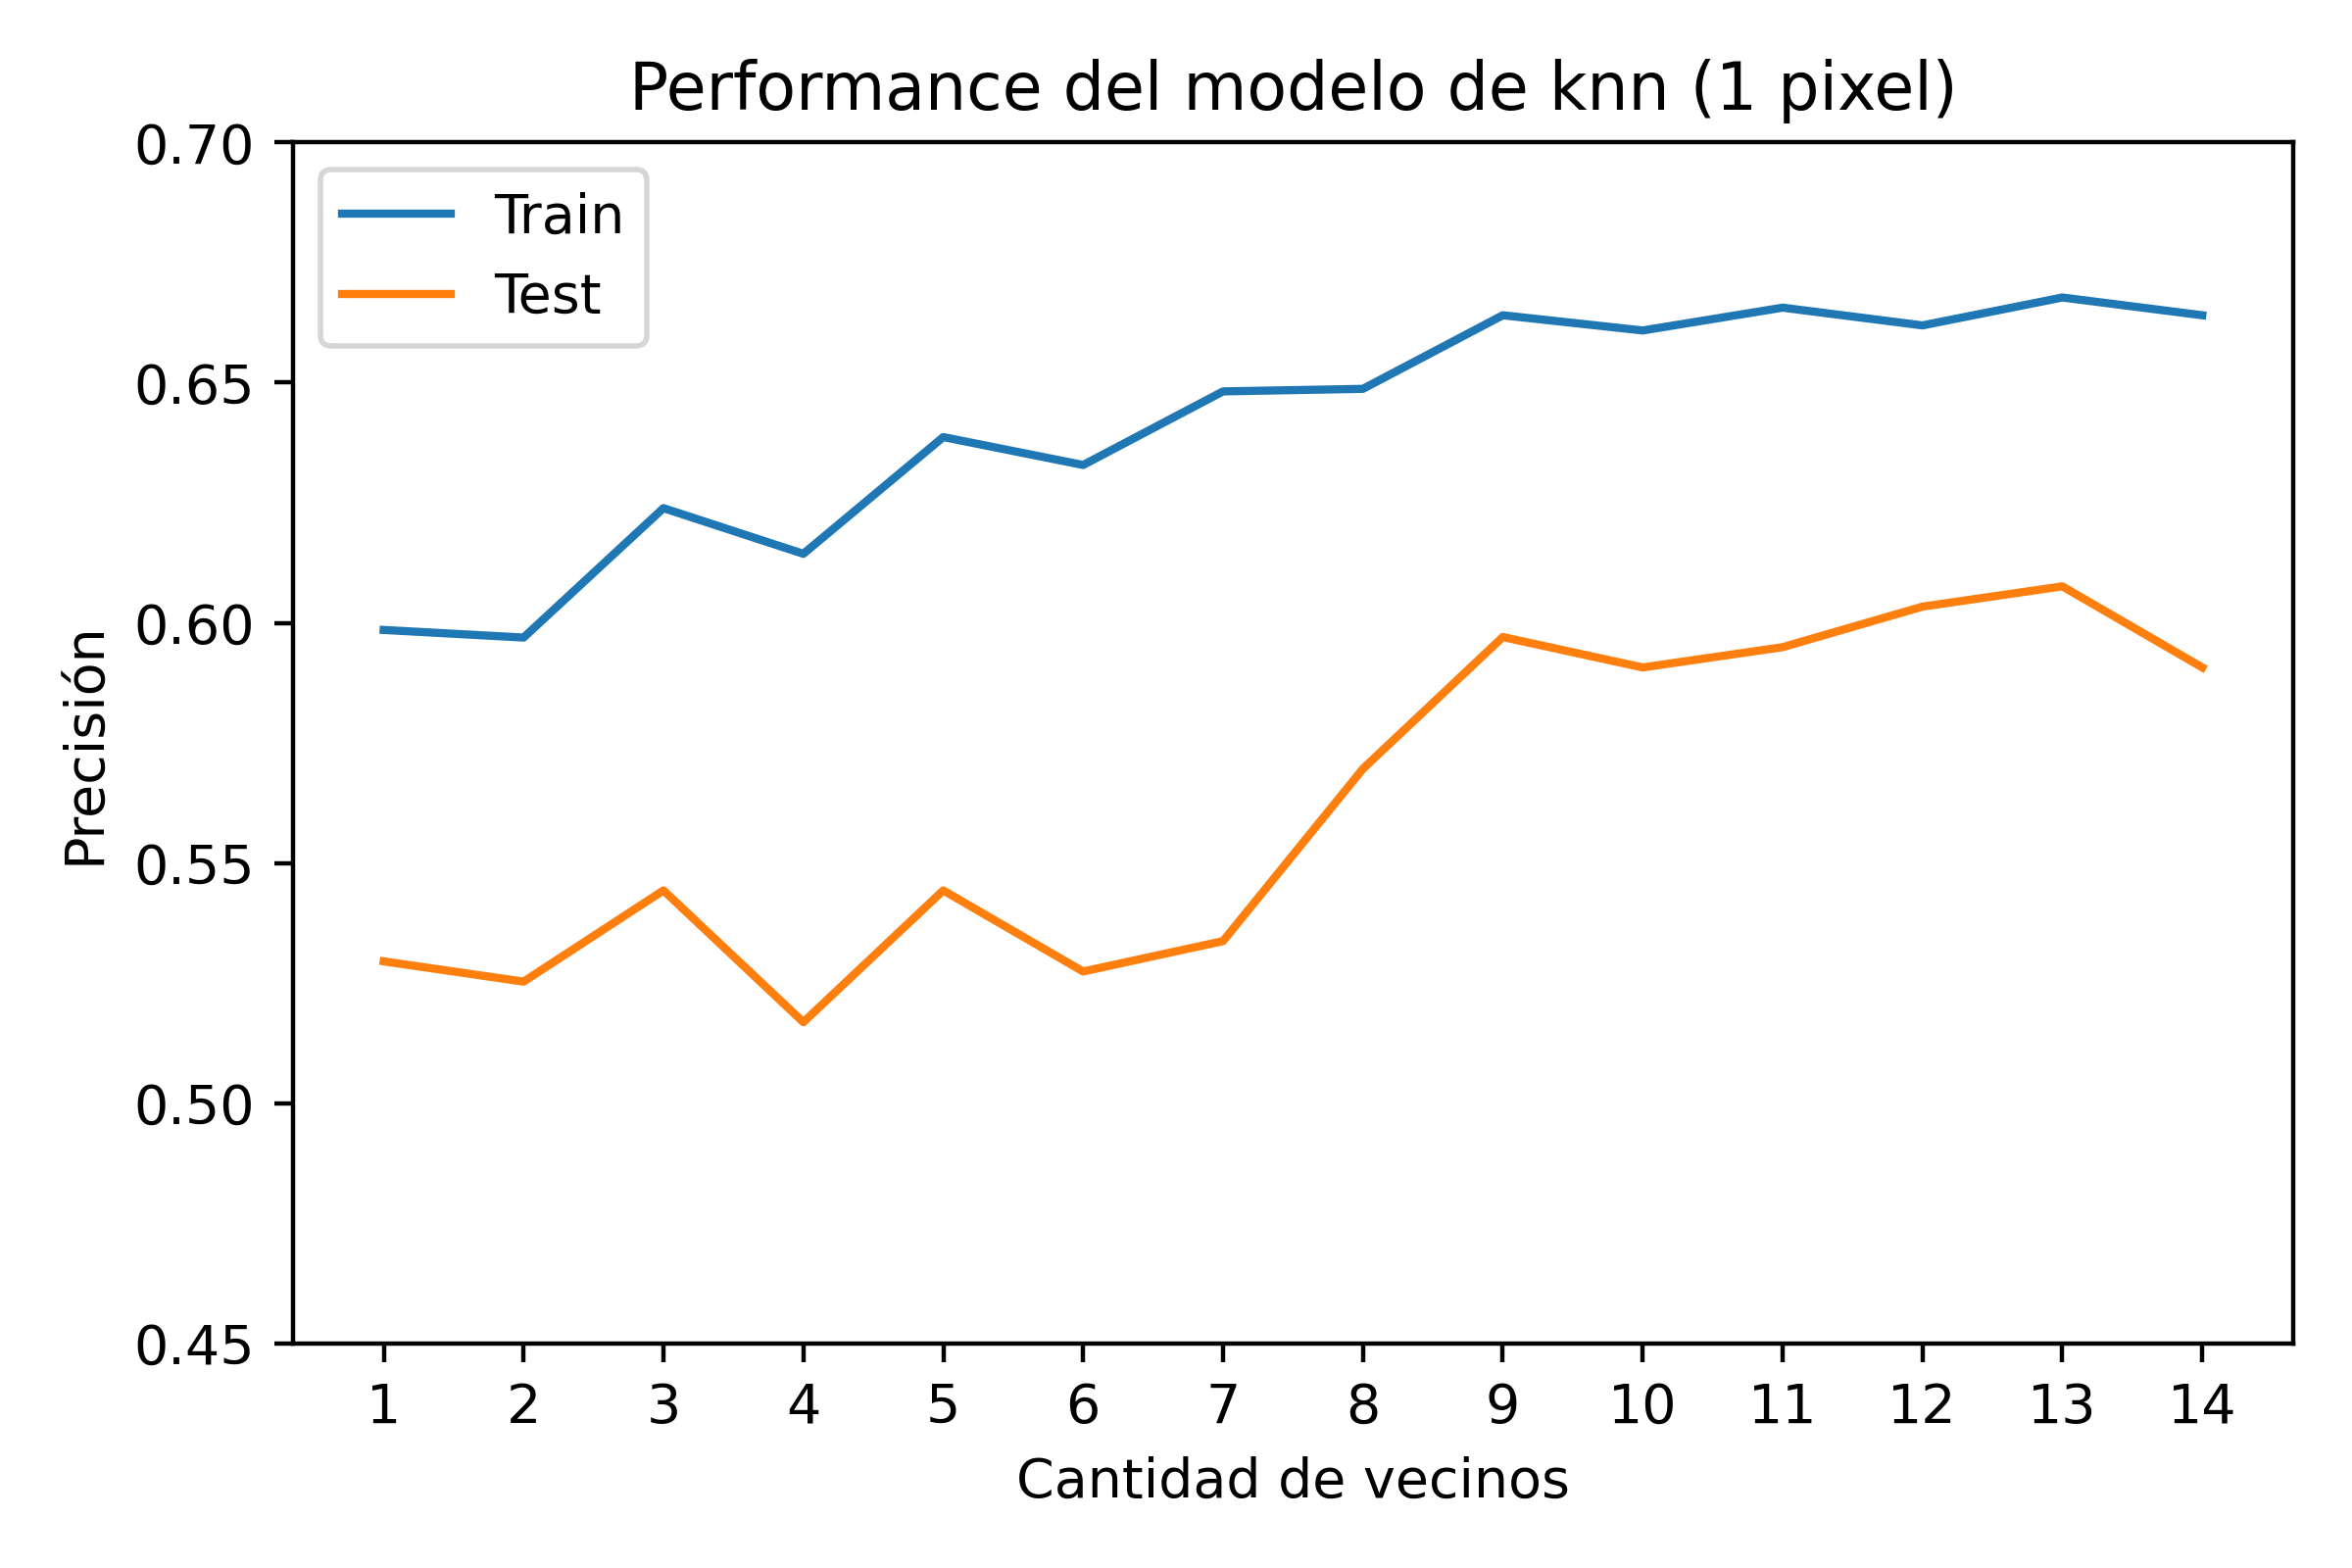
\includegraphics[width=0.9\linewidth]{Imagenes/1pixelbajo.png}
		\caption{Pixeles de baja varianza}
		\label{fig:subfig2}
	\end{subfigure}
	% OJO: el caption siempre va antes del label
	\label{fig:subfigs}
\end{figure}








\end{document}
